% answers.tex —— 2004 年·全国卷Ⅰ·理科 · 参考答案与详细解析片段
% 由 tools/generate_projects.py 依来源总账自 2004/2004_数学真题_全国1理_试题.md + 2004/2004_数学真题_全国1理_解析正文.md + 2004/2004_数学真题_全国1理_答案要点.md 生成，勿手改（改源 MD 后重跑）


\begin{gktip}
固定源 PDF 为印刷页码 182–183 的两页题面，不附答案。以下解析均依据固定源独立复算；第 20 题图形在 LaTeX 工程中以 TikZ/PGFPlots 矢量源重绘。
\end{gktip}

\begin{answer}
\gksolhead{1}{}

\textbf{题目}：

$(1-i)^2\cdot i=$\mbox{（　　）}

（A）$2-2i$　　（B）$2+2i$　　（C）$-2$　　（D）$2$

\Needspace{4\baselineskip}
\textbf{解析}

$(1-i)^2=-2i$，所以 $(1-i)^2i=2$。

\gkanswer{答案：D}

\end{answer}
\begin{answer}
\gksolhead{2}{}

\textbf{题目}：

已知函数 $f(x)=\lg\dfrac{1-x}{1+x}$，若 $f(a)=b$，则 $f(-a)=$\mbox{（　　）}

（A）$b$　　（B）$-b$　　（C）$\dfrac1b$　　（D）$-\dfrac1b$

\Needspace{4\baselineskip}
\textbf{解析}

\nopagebreak[4]
\[
f(-a)=\lg\frac{1+a}{1-a}
=-\lg\frac{1-a}{1+a}
=-f(a)=-b.
\]

\gkanswer{答案：B}

\end{answer}
\begin{answer}
\gksolhead{3}{}

\textbf{题目}：

已知 $\boldsymbol a\text{、}\boldsymbol b$ 均为单位向量，它们的夹角为 $60^\circ$，那么 $|\boldsymbol a+3\boldsymbol b|=$\mbox{（　　）}

（A）$\sqrt7$　　（B）$\sqrt{10}$　　（C）$\sqrt{13}$　　（D）$4$

\Needspace{4\baselineskip}
\textbf{解析}

\nopagebreak[4]
\[
|\boldsymbol a+3\boldsymbol b|^2
=1+9+6\cos60^\circ=13,
\]

故 $|\boldsymbol a+3\boldsymbol b|=\sqrt{13}$。

\gkanswer{答案：C}

\end{answer}
\begin{answer}
\gksolhead{4}{}

\textbf{题目}：

函数 $y=\sqrt{x-1}+1$（$x\geqslant1$）的反函数是\mbox{（　　）}

（A）$y=x^2-2x+2$（$x<1$）　　（B）$y=x^2-2x+2$（$x\geqslant1$）

（C）$y=x^2-2x$（$x<1$）　　（D）$y=x^2-2x$（$x\geqslant1$）

\Needspace{4\baselineskip}
\textbf{解析}

由 $y=\sqrt{x-1}+1$ 得 $x=(y-1)^2+1=y^2-2y+2$。原函数值域为 $y\geqslant1$，所以反函数为 $y=x^2-2x+2$（$x\geqslant1$）。

\gkanswer{答案：B}

\end{answer}
\begin{answer}
\gksolhead{5}{}

\textbf{题目}：

$\left(2x^3-\dfrac1{\sqrt{x}}\right)^7$ 的展开式中常数项是\mbox{（　　）}

（A）$14$　　（B）$-14$　　（C）$42$　　（D）$-42$

\Needspace{4\baselineskip}
\textbf{解析}

\Needspace{5\baselineskip}
取 $\left(-x^{-1/2}\right)^k$ 后幂为 $21-\dfrac72k$。常数项要求 $k=6$，其系数为

\nopagebreak[4]
\[
\binom76 2(-1)^6=14.
\]

\gkanswer{答案：A}

\end{answer}
\begin{answer}
\gksolhead{6}{}

\textbf{题目}：

设 $A\text{、}B\text{、}I$ 均为非空集合，且满足 $A\subseteq B\subseteq I$，则下列各式中错误的是\mbox{（　　）}

（A）$(\complement_I A)\cup B=I$　　（B）$(\complement_I A)\cup(\complement_I B)=I$

（C）$A\cap(\complement_I B)=\varnothing$　　（D）$(\complement_I A)\cap(\complement_I B)=\complement_I B$

\Needspace{4\baselineskip}
\textbf{解析}

因 $A\subseteq B\subseteq I$，有 $\complement_I B\subseteq\complement_I A$。因此 A、C、D 三式分别由补集关系直接成立；B 式左边等于 $\complement_I A$，不一定等于 $I$，故错误的是 B。

\gkanswer{答案：B}

\end{answer}
\begin{answer}
\gksolhead{7}{}

\textbf{题目}：

椭圆 $\dfrac{x^2}{4}+y^2=1$ 的两个焦点为 $F_1\text{、}F_2$，过 $F_1$ 作垂直于 $x$ 轴的直线与椭圆相交，一个交点为 $P$，则 $|\overline{PF_2}|=$\mbox{（　　）}

（A）$\dfrac{\sqrt3}{2}$　　（B）$\sqrt3$　　（C）$\dfrac72$　　（D）$4$

\Needspace{4\baselineskip}
\textbf{解析}

\Needspace{5\baselineskip}
椭圆焦点为 $(\pm\sqrt3,0)$。过 $F_1=(-\sqrt3,0)$ 的竖直弦交点的纵坐标为 $\pm1/2$，故

\nopagebreak[4]
\[
|PF_2|=\sqrt{(2\sqrt3)^2+\left(\frac12\right)^2}=\frac72.
\]

\gkanswer{答案：C}

\end{answer}
\begin{answer}
\gksolhead{8}{}

\textbf{题目}：

设抛物线 $y^2=8x$ 的准线与 $x$ 轴交于点 $Q$，若过点 $Q$ 的直线 $l$ 与抛物线有公共点，则直线 $l$ 的斜率的取值范围是\mbox{（　　）}

（A）$\left[-\dfrac12,\dfrac12\right]$　　（B）$[-2,2]$　　（C）$[-1,1]$　　（D）$[-4,4]$

\Needspace{4\baselineskip}
\textbf{解析}

准线为 $x=-2$，故 $Q=(-2,0)$。设 $l:y=m(x+2)$，代入 $y^2=8x$ 后判别式为 $64(1-m^2)$。有公共点当且仅当 $|m|\leqslant1$。

\gkanswer{答案：C}

\end{answer}
\begin{answer}
\gksolhead{9}{}

\textbf{题目}：

为了得到函数 $y=\sin\left(2x-\dfrac\pi6\right)$ 的图象，可以将函数 $y=\cos2x$ 的图象\mbox{（　　）}

（A）向右平移 $\dfrac\pi6$ 个单位长度　　（B）向右平移 $\dfrac\pi3$ 个单位长度

（C）向左平移 $\dfrac\pi6$ 个单位长度　　（D）向左平移 $\dfrac\pi3$ 个单位长度

\Needspace{4\baselineskip}
\textbf{解析}

\nopagebreak[4]
\[
\cos\left(2x-\frac{2\pi}{3}\right)
=\sin\left(2x-\frac\pi6\right),
\]

所以应将 $y=\cos2x$ 的图象向右平移 $\pi/3$。

\gkanswer{答案：B}

\end{answer}
\begin{answer}
\gksolhead{10}{}

\textbf{题目}：

已知正四面体 $ABCD$ 的表面积为 $S$，其四个面的中心分别为 $E\text{、}F\text{、}G\text{、}H$。设四面体 $EFGH$ 的表面积为 $T$，则 $\dfrac TS$ 等于\mbox{（　　）}

（A）$\dfrac19$　　（B）$\dfrac49$　　（C）$\dfrac14$　　（D）$\dfrac13$

\Needspace{4\baselineskip}
\textbf{解析}

正四面体各面中心组成的正四面体，其棱长为原棱长的 $1/3$，表面积缩小为原来的 $1/9$。

\gkanswer{答案：A}

\end{answer}
\begin{answer}
\gksolhead{11}{}

\textbf{题目}：

从数字 $1,2,3,4,5$ 中，随机抽取 3 个数字（允许重复）组成一个三位数，其各位数字之和等于 9 的概率为\mbox{（　　）}

（A）$\dfrac{13}{125}$　　（B）$\dfrac{16}{125}$　　（C）$\dfrac{18}{125}$　　（D）$\dfrac{19}{125}$

\Needspace{4\baselineskip}
\textbf{解析}

三位数字从 $1,2,3,4,5$ 中独立选取，共有 $5^3=125$ 种。令各位数字为正整数，和为 9；不加上界时方案数为 $\binom82=28$。某一位至少为 6 的方案数为 $\binom32=3$，三位共扣除 $9$，故符合条件的有 $28-9=19$ 种，概率为 $19/125$。

\gkanswer{答案：D}

\end{answer}
\begin{answer}
\gksolhead{12}{}

\textbf{题目}：

$a^2+b^2=1$，$b^2+c^2=2$，$c^2+a^2=2$，则 $ab+bc+ca$ 的最小值为\mbox{（　　）}

（A）$\sqrt3-\dfrac12$　　（B）$\dfrac12-\sqrt3$　　（C）$-\dfrac12-\sqrt3$　　（D）$\dfrac12+\sqrt3$

\Needspace{4\baselineskip}
\textbf{解析}

\Needspace{5\baselineskip}
由三个平方关系得

\nopagebreak[4]
\[
a^2=b^2=\frac12,\qquad c^2=\frac32.
\]

\Needspace{5\baselineskip}
取 $a,b$ 同号、$c$ 异号时

\nopagebreak[4]
\[
ab+bc+ca=\frac12-\sqrt3.
\]

当 $a,b$ 异号时交叉项 $bc+ca$ 抵消，值为 $-1/2$，故最小值为 $\dfrac12-\sqrt3$。

\gkanswer{答案：B}

\end{answer}
\begin{answer}
\gksolhead{13}{}

\textbf{题目}：

不等式 $|x+2|\geqslant|x|$ 的解集是\gkblank{}。

\Needspace{4\baselineskip}
\textbf{解析}

\nopagebreak[4]
\[
|x+2|\geqslant|x|
\Longleftrightarrow
(x+2)^2\geqslant x^2
\Longleftrightarrow x\geqslant-1.
\]

\gkanswer{答案：$[-1,+\infty)$}

\end{answer}
\begin{answer}
\gksolhead{14}{}

\textbf{题目}：

由动点 $P$ 向圆 $x^2+y^2=1$ 引两条切线 $PA\text{、}PB$，切点分别为 $A\text{、}B$，$\angle APB=60^\circ$，则动点 $P$ 的轨迹方程为\gkblank{}。

\Needspace{4\baselineskip}
\textbf{解析}

与第 15 题相同，切线构成的直角三角形给出 $OP=2$，所以轨迹方程为 $x^2+y^2=4$。

\gkanswer{答案：$x^2+y^2=4$}

\end{answer}
\begin{answer}
\gksolhead{15}{}

\textbf{题目}：

\Needspace{5\baselineskip}
已知数列 $\{a_n\}$，满足 $a_1=1$，

\nopagebreak[4]
\[
a_n=a_1+2a_2+3a_3+\cdots+(n-1)a_{n-1}\quad(n\geqslant2)\text{，}
\]

\Needspace{5\baselineskip}
则 $\{a_n\}$ 的通项 $a_n=$

\nopagebreak[4]
\[
\begin{cases}
1,&n=1,\\
\rule{3em}{0.4pt},&n\geqslant2.
\end{cases}
\]

\Needspace{4\baselineskip}
\textbf{解析}

\Needspace{5\baselineskip}
由递推式

\nopagebreak[4]
\[
a_{n+1}=a_1+2a_2+\cdots+na_n=(n+1)a_n,
\]

\Needspace{5\baselineskip}
其中最后一步使用 $a_n=a_1+2a_2+\cdots+(n-1)a_{n-1}$。又 $a_2=1$，故

\nopagebreak[4]
\[
a_n=2\cdot3\cdots n=\frac{n!}{2}\quad(n\geqslant2),
\]

并且 $a_1=1$。

\gkanswer{答案：$a_1=1$，且 $a_n=\dfrac{n!}{2}\ (n\geqslant2)$}

\end{answer}
\begin{answer}
\gksolhead{16}{}

\textbf{题目}：

已知 $\boldsymbol a\text{、}\boldsymbol b$ 为不垂直的异面直线，$\alpha$ 是一个平面，则 $\boldsymbol a\text{、}\boldsymbol b$ 在 $\alpha$ 上的射影有可能是：

① 两条平行直线；

② 两条互相垂直的直线；

③ 同一条直线；

④ 一条直线及其外一点。

在上面结论中，正确结论的编号是\gkblank{}。（写出所有正确结论的编号）

\Needspace{4\baselineskip}
\textbf{解析}

与平面的正投影可以构造为两条平行直线、两条互相垂直的直线，或一条直线和一个外点，所以 ①、②、④ 可能。

若投影为同一条直线，则两条原直线都位于该投影直线的正投影逆像平面内，从而共面，不可能是异面直线。因此正确编号为 ①②④。

\gkanswer{答案：①②④}

\end{answer}
\begin{answer}
\gksolhead{17}{}

\textbf{题目}：

\Needspace{5\baselineskip}
求函数

\nopagebreak[4]
\[
f(x)=\frac{\sin^4x+\cos^4x+\sin^2x\cos^2x}{2-\sin2x}
\]

的最小正周期、最大值和最小值。

\Needspace{4\baselineskip}
\textbf{解析}

\Needspace{5\baselineskip}
记 $s=\sin2x$，则

\nopagebreak[4]
\[
\sin^4x+\cos^4x+\sin^2x\cos^2x
=1-\frac{s^2}{4}
=\frac{(2-s)(2+s)}4.
\]

所以 $f(x)=\dfrac12+\dfrac14\sin2x$，最小正周期为 $\pi$，最大值为 $3/4$，最小值为 $1/4$。

\gkanswer{答案：最小正周期为 $\pi$，最大值为 $\dfrac34$，最小值为 $\dfrac14$}

\end{answer}
\begin{answer}
\gksolhead{18}{}

\textbf{题目}：

一接待中心有 $A\text{、}B\text{、}C\text{、}D$ 四部热线电话，已知某一时刻电话 $A\text{、}B$ 占线的概率均为 $0.5$，电话 $C\text{、}D$ 占线的概率均为 $0.4$，各部电话是否占线相互之间没有影响。假设该时刻有 $\xi$ 部电话占线。试求随机变量 $\xi$ 的概率分布和它的期望。

\Needspace{4\baselineskip}
\textbf{解析}

\Needspace{5\baselineskip}
记电话 $A\text{、}B$ 的占线概率为 $1/2$，电话 $C\text{、}D$ 的占线概率为 $2/5$。概率生成函数为

\nopagebreak[4]
\[
\left(\frac12+\frac12t\right)^2
\left(\frac35+\frac25t\right)^2.
\]

\Needspace{5\baselineskip}
展开得

\nopagebreak[4]
\[
\begin{array}{c|ccccc}
\xi&0&1&2&3&4\\
\hline
P&\dfrac9{100}&\dfrac3{10}&\dfrac{37}{100}&\dfrac15&\dfrac1{25}
\end{array}
\]

\Needspace{5\baselineskip}
因此

\nopagebreak[4]
\[
E\xi=0\cdot\frac9{100}+1\cdot\frac3{10}
+2\cdot\frac{37}{100}+3\cdot\frac15+4\cdot\frac1{25}
=\frac95.
\]

\gkanswer{答案：$P(\xi=0,1,2,3,4)=\left(\dfrac9{100},\dfrac3{10},\dfrac{37}{100},\dfrac15,\dfrac1{25}\right)$，且 $E\xi=\dfrac95$}

\end{answer}
\begin{answer}
\gksolhead{19}{}

\textbf{题目}：

已知 $a\in\mathbb R$，求函数 $f(x)=x^2e^{ax}$ 的单调区间。

\Needspace{4\baselineskip}
\textbf{解析}

\nopagebreak[4]
\[
f'(x)=e^{ax}(2x+ax^2)=e^{ax}x(2+ax).
\]

因 $e^{ax}>0$，只需讨论 $x(2+ax)$ 的符号：

\begin{itemize}
\item $a>0$ 时，临界点为 $-2/a<0$，在 $\left(-\infty,-2/a\right)$ 与 $(0,+\infty)$ 上递增，在 $\left(-2/a,0\right)$ 上递减；
\item $a=0$ 时，$f(x)=x^2$，在 $(-\infty,0)$ 上递减，在 $(0,+\infty)$ 上递增；
\item $a<0$ 时，临界点为 $-2/a>0$，在 $(-\infty,0)$ 与 $\left(-2/a,+\infty\right)$ 上递减，在 $\left(0,-2/a\right)$ 上递增。
\end{itemize}

\gkanswer{答案：$a>0$ 时增区间为 $\left(-\infty,-\dfrac2a\right)\cup(0,+\infty)$、减区间为 $\left(-\dfrac2a,0\right)$；$a=0$ 时减区间为 $(-\infty,0)$、增区间为 $(0,+\infty)$；$a<0$ 时减区间为 $(-\infty,0)\cup\left(-\dfrac2a,+\infty\right)$、增区间为 $\left(0,-\dfrac2a\right)$}

\end{answer}
\begin{answer}
\gksolhead{20}{}

\textbf{题目}：

如图，已知四棱锥 $P-ABCD$，$PB\perp AD$，侧面 $PAD$ 为边长等于 2 的正三角形，底面 $ABCD$ 为菱形，侧面 $PAD$ 与底面 $ABCD$ 所成的二面角为 $120^\circ$。
\nopagebreak[4]
\begin{center}% 2004 年全国卷Ⅰ理科第 20 题：四棱锥
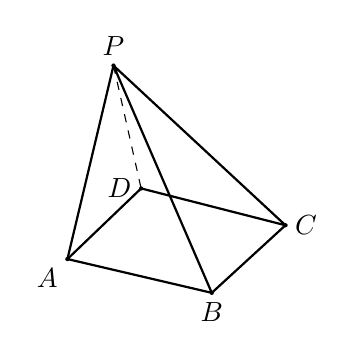
\begin{tikzpicture}[>=stealth,scale=0.78]
  \coordinate (A) at (0,0); \coordinate (B) at (2.35,-0.55);
  \coordinate (C) at (3.55,0.55); \coordinate (D) at (1.2,1.15);
  \coordinate (P) at (0.75,3.15);
  \draw[thick] (A)--(B)--(C)--(D)--cycle;
  \draw[thick] (P)--(A) (P)--(B) (P)--(C);
  \draw[dashed] (P)--(D);
  \fill (P) circle (1pt) node[above] {$P$};
  \fill (A) circle (1pt) node[below left] {$A$};
  \fill (B) circle (1pt) node[below] {$B$};
  \fill (C) circle (1pt) node[right] {$C$};
  \fill (D) circle (1pt) node[left] {$D$};
\end{tikzpicture}
\end{center}
\nopagebreak[4]
（1） 求点 $P$ 到平面 $ABCD$ 的距离；

（2） 求面 $APB$ 与面 $CPB$ 所成二面角的大小。

\Needspace{4\baselineskip}
\textbf{解析}

\gksubpart{(1)}

\Needspace{5\baselineskip}
取

\nopagebreak[4]
\[
A=(0,0,0),\quad D=(2,0,0),\quad B=(1,\sqrt3,0),\quad C=(3,\sqrt3,0),
\]

\Needspace{5\baselineskip}
并由侧面正三角形、底面二面角 $120^\circ$ 及 $PB\perp AD$ 得

\nopagebreak[4]
\[
P=\left(1,-\frac{\sqrt3}{2},\frac32\right).
\]

\Needspace{5\baselineskip}
故点 $P$ 到底面的距离为 $3/2$。对公共棱 $PB$，取

\nopagebreak[4]
\[
\boldsymbol n_1=\overrightarrow{AB}\times\overrightarrow{AP}
=\left(\frac{3\sqrt3}{2},-\frac32,-\frac{3\sqrt3}{2}\right),
\]

\nopagebreak[4]
\[
\boldsymbol n_2=\overrightarrow{BC}\times\overrightarrow{BP}
=(0,-3,-3\sqrt3).
\]

\gksubpart{(2)}

\Needspace{5\baselineskip}
于是两平面的锐角夹角 $\theta$ 满足

\nopagebreak[4]
\[
\cos\theta
=\frac{|\boldsymbol n_1\cdot\boldsymbol n_2|}
{|\boldsymbol n_1||\boldsymbol n_2|}
=\frac{2\sqrt7}{7}.
\]

\gkanswer{答案（1）：点 $P$ 到平面 $ABCD$ 的距离为 $\dfrac32$}

\gkanswer{答案（2）：两平面的锐角夹角 $\theta$ 满足 $\cos\theta=\dfrac{2\sqrt7}{7}$，即 $\theta=\arccos\dfrac{2\sqrt7}{7}$；若取棱锥内部二面角，则为 $\pi-\theta$}

\end{answer}
\begin{answer}
\gksolhead{21}{}

\textbf{题目}：

已知双曲线 $C:\dfrac{x^2}{a^2}-y^2=1$（$a>0$）与直线 $l:x+y=1$ 相交于两个不同的点 $A\text{、}B$。

（1） 求双曲线 $C$ 的离心率 $e$ 的取值范围；

（2） 设直线 $l$ 与 $y$ 轴的交点为 $P$，且 $\overrightarrow{PA}=\dfrac5{12}\overrightarrow{PB}$。求 $a$ 的值。

\Needspace{4\baselineskip}
\textbf{解析}

\gksubpart{(1)}

\Needspace{5\baselineskip}
代入 $y=1-x$ 得

\nopagebreak[4]
\[
\left(\frac1{a^2}-1\right)x^2+2x-2=0.
\]

\Needspace{5\baselineskip}
两个不同交点要求 $a\ne1$ 且

\nopagebreak[4]
\[
4\left(\frac2{a^2}-1\right)>0,
\]

\Needspace{5\baselineskip}
即 $0<a<\sqrt2$ 且 $a\ne1$。双曲线离心率

\nopagebreak[4]
\[
e=\frac{\sqrt{a^2+1}}a
\]

随 $a$ 增大而减小，故 $e>\sqrt6/2$ 且 $e\ne\sqrt2$。

\gksubpart{(2)}

\Needspace{5\baselineskip}
第二问与直线上的横坐标参数相同。若两交点横坐标为 $r,s$，由 $\overrightarrow{PA}=\dfrac5{12}\overrightarrow{PB}$ 有 $r=\dfrac5{12}s$。又根和等于根积，所以

\nopagebreak[4]
\[
r+s=rs,\qquad r=\frac5{12}s,
\]

\Needspace{5\baselineskip}
解得 $r=17/12$、$s=17/5$。因此 $r+s=289/60$，而根和又为 $-2a^2/(1-a^2)$，从而

\nopagebreak[4]
\[
-\frac{2a^2}{1-a^2}=\frac{289}{60}
\Longrightarrow a=\frac{17}{13}.
\]

\gkanswer{答案（1）：$e\in\left(\dfrac{\sqrt6}{2},+\infty\right)\setminus\{\sqrt2\}$}

\gkanswer{答案（2）：$a=\dfrac{17}{13}$}

\end{answer}
\begin{answer}
\gksolhead{22}{}

\textbf{题目}：

\Needspace{5\baselineskip}
已知数列 $\{a_n\}$ 中，$a_1=1$，且

\nopagebreak[4]
\[
a_{2k}=a_{2k-1}+(-1)^k,\qquad a_{2k+1}=a_{2k}+3^k,\qquad k=1,2,3,\cdots\text{。}
\]

（1） 求 $a_3\text{、}a_5$；

（2） 求 $\{a_n\}$ 的通项公式。

\Needspace{4\baselineskip}
\textbf{解析}

\gksubpart{(1)}

\Needspace{5\baselineskip}
由递推式

\nopagebreak[4]
\[
a_2=a_1+(-1)^1=0,\qquad a_3=a_2+3^1=3,
\]

\Needspace{5\baselineskip}
以及

\nopagebreak[4]
\[
a_4=a_3+(-1)^2=4,\qquad a_5=a_4+3^2=13.
\]

\gksubpart{(2)}

\Needspace{5\baselineskip}
对 $k\geqslant0$，逐对相加可得

\nopagebreak[4]
\[
a_{2k+1}=1+\sum_{j=1}^k\left((-1)^j+3^j\right)
=\frac{3^{k+1}+(-1)^k-2}{2}.
\]

\Needspace{5\baselineskip}
再由 $a_{2k}=a_{2k-1}+(-1)^k$ 得

\nopagebreak[4]
\[
a_{2k}=\frac{3^k+(-1)^k-2}{2}.
\]

将 $k$ 分别换成 $n/2$ 和 $(n-1)/2$，即得答案中的分段通项。

\gkanswer{答案（1）：$a_3=3$，$a_5=13$}

\gkanswer{答案（2）：偶数 $n=2k$ 时 $a_n=\dfrac{3^k+(-1)^k-2}{2}$；奇数 $n=2k+1$ 时 $a_n=\dfrac{3^{k+1}+(-1)^k-2}{2}$}

\end{answer}